\documentclass[times, 10pt,twocolumn]{article} 
\usepackage{mapnoreduce-report-g03}
\usepackage{times}
\usepackage{graphicx}
\usepackage[utf8x]{inputenc}
\usepackage{enumitem}
\usepackage{amsmath}
\usepackage{bm}
\usepackage{wasysym}
\usepackage{amsfonts}%
\usepackage{amssymb}%
\usepackage{graphicx}
\usepackage{fixltx2e}
\usepackage{color} 
\usepackage{colortbl}
\usepackage{subfig}
\usepackage{url}
\usepackage{cite}
\usepackage[portuguese, english]{babel} 
\usepackage{threeparttable}
\PassOptionsToPackage{hyphens}{url}\usepackage{hyperref}
\usepackage[hyphens]{url}\hypersetup{breaklinks=true}
\usepackage[square,sort,comma,numbers]{natbib}
\usepackage{tabularx}
\usepackage{booktabs}
\usepackage{chngpage}
\usepackage{pdflscape}
\usepackage[table]{xcolor}
\definecolor{lightgray}{gray}{0.9}
\usepackage{tikz}
\usepackage[printonlyused,nolist]{acronym}

\pagestyle{empty}

\begin{document}
	\title{MapNoReduce Platform}
	
	\author{
        João Pinho\\jpe.pinho@gmail.com\and Diogo Rosa\\
        diogo.m.c.rosa@gmail.com\and Cláudia Filipe\\
        claudia.p.b.filipe@gmail.com\\\\		 
		Instituto Superior Técnico\\
        Middleware for Distributed Internet Applications\\
        Lisbon, Portugal
    }
	\maketitle
	\thispagestyle{empty}
	
    % region:acronyms { %
    \acrodef{MNRP}{MapNoReduce Platform}
    % } %
    
	\begin{abstract}
		This project consists in the design and implementation of \ac{MNRP}, a simplified implementation of the MapReduce middleware and programming model. This platform extracts the input key/value pairs from input files and distributes the Map calls, called Jobs, across multiple machines, the Workers. 
		Also, the platform ensures a good performance by monitoring job's progress, detecting faulty or slow machines and rescheduling their tasks on idle machines. That is assured by Job Trackers, which are distributed in this platform, in contrast to the original implementation of MapReduce, where they are centralized. This mechanism was implemented inspired in Facebook's solution—Corona~\cite{ChingFacebook2012}. 
		Additionally, in order to test the platform it was developed a PuppetMaster component which allows to control the platform, and also to induce some delays and faults to the system in order to perform some tests and evaluation.
	\end{abstract}
    
	\section{Introduction}
	MapReduce was introduced by Google in 2004~\cite{GhemawatMR2008} and is currently one of the most popular approaches for large scale data analytics - also thanks to the availability of high quality open-source implementations. When using the MapReduce paradigm, the computation takes a set of input key/value pairs, and produces a set of output key/value pairs. MapReduce users express the computation as two functions: Map and Reduce. 
	This project focuses only the Map part, which uses a Map function given by the user and an input set of key/value pairs to produce a set of key/value pairs. 
	In \ac{MNRP} the keys are the numbers of the line of the file being read and the values are the content of those lines.
    The Map invocations, called Jobs, are distributed across multiple machines by automatically partitioning the input data into a set of splits of size S. The input splits can be processed in parallel by those machines, named Workers. The system ensures that for each job submitted, all the input data is processed with a good performance through the monitoring of jobs' progress, fault or slow machines detection and reschedule of idle machine's tasks.
	In the original MapReduce implementation these tasks are performed by the JobTracker which is a centralized component. If the JobTracker fails the system can't receive new jobs nor processing pending ones, which can be critical in systems that need high availability.
	Considering JobTracker as a single point of failure~\cite{Kalavri2013}, it is necessary to replicate this component. As it would add complexity to the system and overhead, this project also introduces a new entity, the CoordinationManager, separating cluster resource management from job coordination, which allows the system to focus on make faster scheduling tasks.  
	
	\section{MapNoReduce Architecture}
		
        \ac{MNRP} is a simplified implementation of the MapReduce middleware and programming model, focused on the Map part. On this simplified version, our work provides a solution to common problems related with the reference architecture of the MapReduce platform. Those problems are related with fault-tolerance, replication and performance and will be discussed in the next sections. Additionally, we added some features that enable the overall testing of the system, such as the ability to run scripts over one or more functional servers or the capacity to monitor the system state while running those scripts.
        
        \begin{figure}[!h]
            \begin{center}
                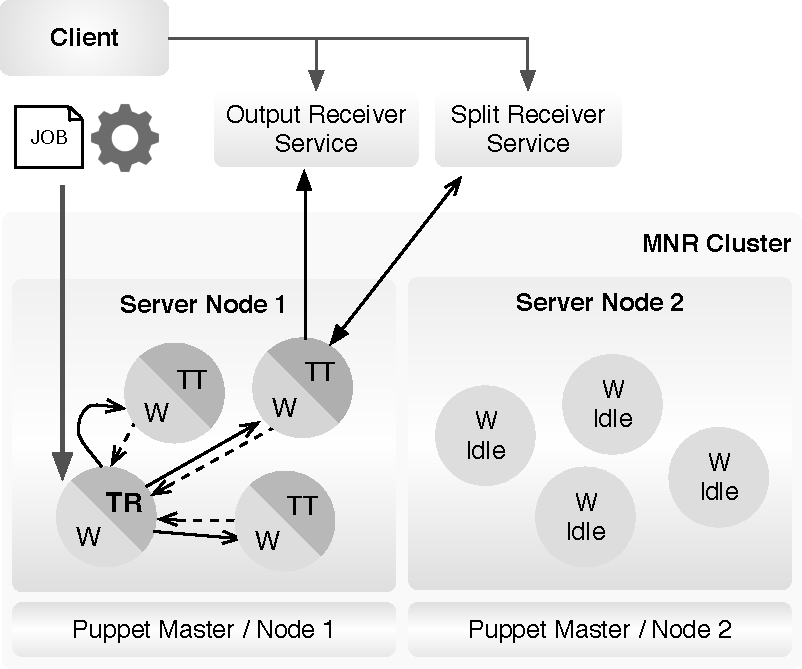
\includegraphics[width=0.48\textwidth]{pics/architecture.pdf}
                \caption{We illustrate an example of the MapNoReduce architecture. We represent one cluster with two server nodes. Inside the processing node, one JobTracker coordinates with other TaskTrackers to process the client job.  }
                \label{fig:mnr-architecture}
            \end{center}
        \end{figure}
        
    	\subsection{Worker}
        %What is it? Why is it necessary? What are their functions? Final conclusion, to close section.
        
        In \ac{MNRP}, workers are simple .NET Remoting Services that receive requests on a given endpoint, known as \textit{Service URI}. 
        
        Every time a job gets submitted to the \ac{MNRP}, an entry worker gets selected to handle its processing. Workers are therefore, available working units that in a given \textit{Server Node} represent its work capacity. This is, for a given server node with 10 workers, such node has capacity to parallelize work to 10 workers.
        
        The \textit{Service URI} of a worker is composed by 4 parts, starting with the protocol, followed by the \textit{host name}, the \textit{host port}, and finally the worker identifier. An example of such a \textit{Service URI} would be something like \textit{tcp://192.168.1.74:20001/W1}, representing the endpoint for the worker 1 in the server node.
        
        It is also worth mentioning that, since a worker is no more than a thread waiting for requests on a given server node — represented by a physical machine, — workers share the same machine resources among them when running in parallel, if all located in the same server node obviously.
        
        When a worker gets selected by a client application as entry worker, it is made responsible for the correct processing of that job. This means that it must keep track of all the splits that must be processed for that job, what is their status, whose worker is processing each split and in case of a failure it must reassign the lost split to another worker, re-executing the job split if necessary.
        
        On the other end, each worker that receives the job of processing a given job's split, must report progress to the entry worker in regular intervals, to let it know that the job split is being processed without any problems.
        
        In the \ac{MNRP}, to an entry worker responsible of managing the processing of a whole job we call, Task Runner and to a worker that reports progress to the Task Runner we call Task Tracker.
       
    	\subsection{Job Tracker}
        %What is it? Why is it necessary? What are their functions? Final conclusion, to close section.
        
        The overall execution and progress tracking of a job is handled by Job Trackers. In \ac{MNRP} \textit{Job Trackers} can have two distinct functions, they could be responsible for the distribution of splits for a given job, or they could be responsible for reporting progress about the processing of a given split.
            
        
        
               
            \subsubsection{Task Runner}
    
            \subsubsection{Task Tracker}
    
        	\subsubsection{Job Scheduler}
        
        \subsection{Replication}
        
        	\subsubsection{Coordination Manager}
        	
        	\subsubsection{Slave Replica}
    	
    	\subsection{Cluster Resource Management}
    	
            \subsubsection{Fair Share Scheduler}
        
    	\subsection{Puppet Master}
        
            \subsubsection{Management Interface}
            
            \subsubsection{Create Worker}
            
            \subsubsection{Status}
                	
            \subsubsection{Wait}
            
            \subsubsection{Slow Worker}
            
            \subsubsection{Freeze/Unfreeze Worker}
            
            \subsubsection{Freeze/Unfreeze Communication}
	
	\section{Evaluation}
	
	\section{Conclusions}
	
	\bibliographystyle{mapnoreduce-report-g03}
	\bibliography{mapnoreduce-rpt-g03}
\end{document}